\documentclass[border=5mm]{standalone}
\usepackage{tikz}
\usepackage{tikz-3dplot}
\usetikzlibrary{bending}
\usetikzlibrary{quotes,angles,positioning}

\begin{document}

% DEFINE 3D COORDINATE FRAME (using tikz-3dplot)
% Will set the orientation of x,y,z
% Syntax: \tdplotsetdisplay{\theta_d}{\phi_d}
\tdplotsetmaincoords{70}{100}

% SET SOME VARIABLES
\pgfmathsetmacro{\sphereRadius}{1}


% USE tdplot_main_coords FOR YOUR DEFINED 3D COORDINATE FRAME
% Coordinate transformation provided by tikz-3dplot
\begin{tikzpicture}[scale=6,tdplot_main_coords]

    % SPHERE
    \shadedraw[tdplot_screen_coords, ball color = white] (0,0) circle (\sphereRadius);

    % X, Y, Z AXIS
    \draw[thick,->] (0,0,0) -- (1.7,0,0) node[anchor=north east] {$x$};
    \draw[thick,->] (0,0,0) -- (0,1.7,0) node[anchor=north west] {$y$};
    \draw[thick,->] (0,0,-1.7) -- (0,0,1.7) node[anchor=south] {$z$};

    % DOTS ON AXIS CROSSING SPHERE
    \coordinate (coordX) at (\sphereRadius,0,0);
    \coordinate (coordY) at (0,\sphereRadius,0);
    \coordinate (coordZ) at (0,0,\sphereRadius);
    \node at (coordX) [circle, color=green, fill,inner sep=1.5pt] {};
    \node at (coordX) [color=black, below right = 1mm of coordX] {$Hi Jeff$};
    \node at (coordY) [circle,color=green,fill,inner sep=1.5pt]{};
    \node at (coordZ) [circle,fill,inner sep=1.5pt]{};

    %LABEL DOTS ON AXIS CROSSING SPHERE

    % CELESTIAL EQUATOR
    \draw[dashed, thick, color=green] (\sphereRadius,0,0) arc (0:360:\sphereRadius);
    \draw[thick, color=green] (\sphereRadius,0,0) arc (0:110:\sphereRadius);
    \draw[thick, color=green] (\sphereRadius,0,0) arc (0:-70:\sphereRadius);

    % LABEL CELESTIAL EQUATOR

    % EARTH
    \draw[thick] (0,0) circle (0.1cm);
    \shade[ball color=blue!60!white,opacity=0.80] (0,0) circle (0.1cm);


\end{tikzpicture}

%Angle Definitions
%-----------------
 
%set the plot display orientation
%synatax: \tdplotsetdisplay{\theta_d}{\phi_d}
\tdplotsetmaincoords{65}{110}
\pgfmathsetmacro{\rvec}{1.2}
\pgfmathsetmacro{\thetavecc}{55}
\pgfmathsetmacro{\phivecc}{35} 
\pgfmathsetmacro{\thetaveccc}{39.7}
\pgfmathsetmacro{\phiveccc}{55}
 
 
\begin{tikzpicture}[scale=6,tdplot_main_coords]
    
    \shadedraw[tdplot_screen_coords,ball color = white] (0,0) circle (\rvec);

    %-----------------------
    \coordinate (O) at (0,0,0);
    
    \tdplotsetcoord{B}{\rvec}{\thetavecc}{\phivecc}
    \tdplotsetcoord{C}{\rvec}{\thetaveccc}{\phiveccc}
    
    %draw the main coordinate system axes
    \draw[thick,->] (0,0,0) -- (1.7,0,0) node[anchor=north east]{$x$};
    \draw[thick,->] (0,0,0) -- (0,1.7,0) node[anchor=north west]{$y$};
    \draw[thick,->] (0,0,0) -- (0,0,1.7) node[anchor=south]{$z$};
    
    \draw[-stealth,very thick,color=blue] (O) -- (B);
    
    \draw[-stealth,very thick,color=green!60!black] (O) -- (C);
    
    \draw[dashed, color=blue] (O) -- (Bxy);
    \draw[dashed, color=blue] (B) -- (Bxy);
    
    \draw[dashed, color=green!60!black] (O) -- (Cxy);
    \draw[dashed, color=green!60!black] (C) -- (Cxy);
    
    \tdplotdrawarc[color=blue]{(O)}{0.3}{0}{\phivecc}{anchor=north}{$\lambda_A$}
    
    \tdplotsetthetaplanecoords{\phivecc}
    
    \tdplotdrawarc[color=blue,tdplot_rotated_coords]{(0,0,0)}{0.3}{90}{\thetavecc}{anchor=south west}{$\varphi_A$}
    
    \tdplotdrawarc[color=green!40!black]{(O)}{0.7}{0}{\phiveccc}{anchor=north}{$\lambda_B$}
    
    \tdplotsetthetaplanecoords{\phiveccc}
    
    \tdplotdrawarc[color=green!40!black,tdplot_rotated_coords]{(0,0,0)}{0.7}{90}{\thetaveccc}{anchor=south west}{$\varphi_B$}
    
    \draw[dashed] (\rvec,0,0) arc (0:360:\rvec);
    \draw[thick] (\rvec,0,0) arc (0:110:\rvec);
    \draw[thick] (\rvec,0,0) arc (0:-70:\rvec);
    
    \tdplotsetthetaplanecoords{35}
    \draw[thick,tdplot_rotated_coords] (\rvec,0,0) arc (0:151:\rvec);
    \draw[very thick,color=red,tdplot_rotated_coords] (\rvec,0,0) arc (0:55:\rvec);
    \draw[dashed,tdplot_rotated_coords] (\rvec,0,0) arc (180:-40:-\rvec);
    \draw[thick,tdplot_rotated_coords] (\rvec,0,0) arc (360:336:\rvec);
    
    \tdplotsetthetaplanecoords{55}
    \draw[thick,tdplot_rotated_coords] (\rvec,0,0) arc (0:147:\rvec);
    \draw[very thick,color=red,tdplot_rotated_coords] (\rvec,0,0) arc (0:40:\rvec);
    \draw[dashed,tdplot_rotated_coords] (\rvec,0,0) arc (180:-40:-\rvec);
    \draw[thick,tdplot_rotated_coords] (\rvec,0,0) arc (360:334:\rvec);
    
    \tdplotsetrotatedcoords{-79.1}{-120}{27.3}
    \draw[very thick,color=red,tdplot_rotated_coords] (\rvec,0,0) arc (0:21:\rvec);

\end{tikzpicture}

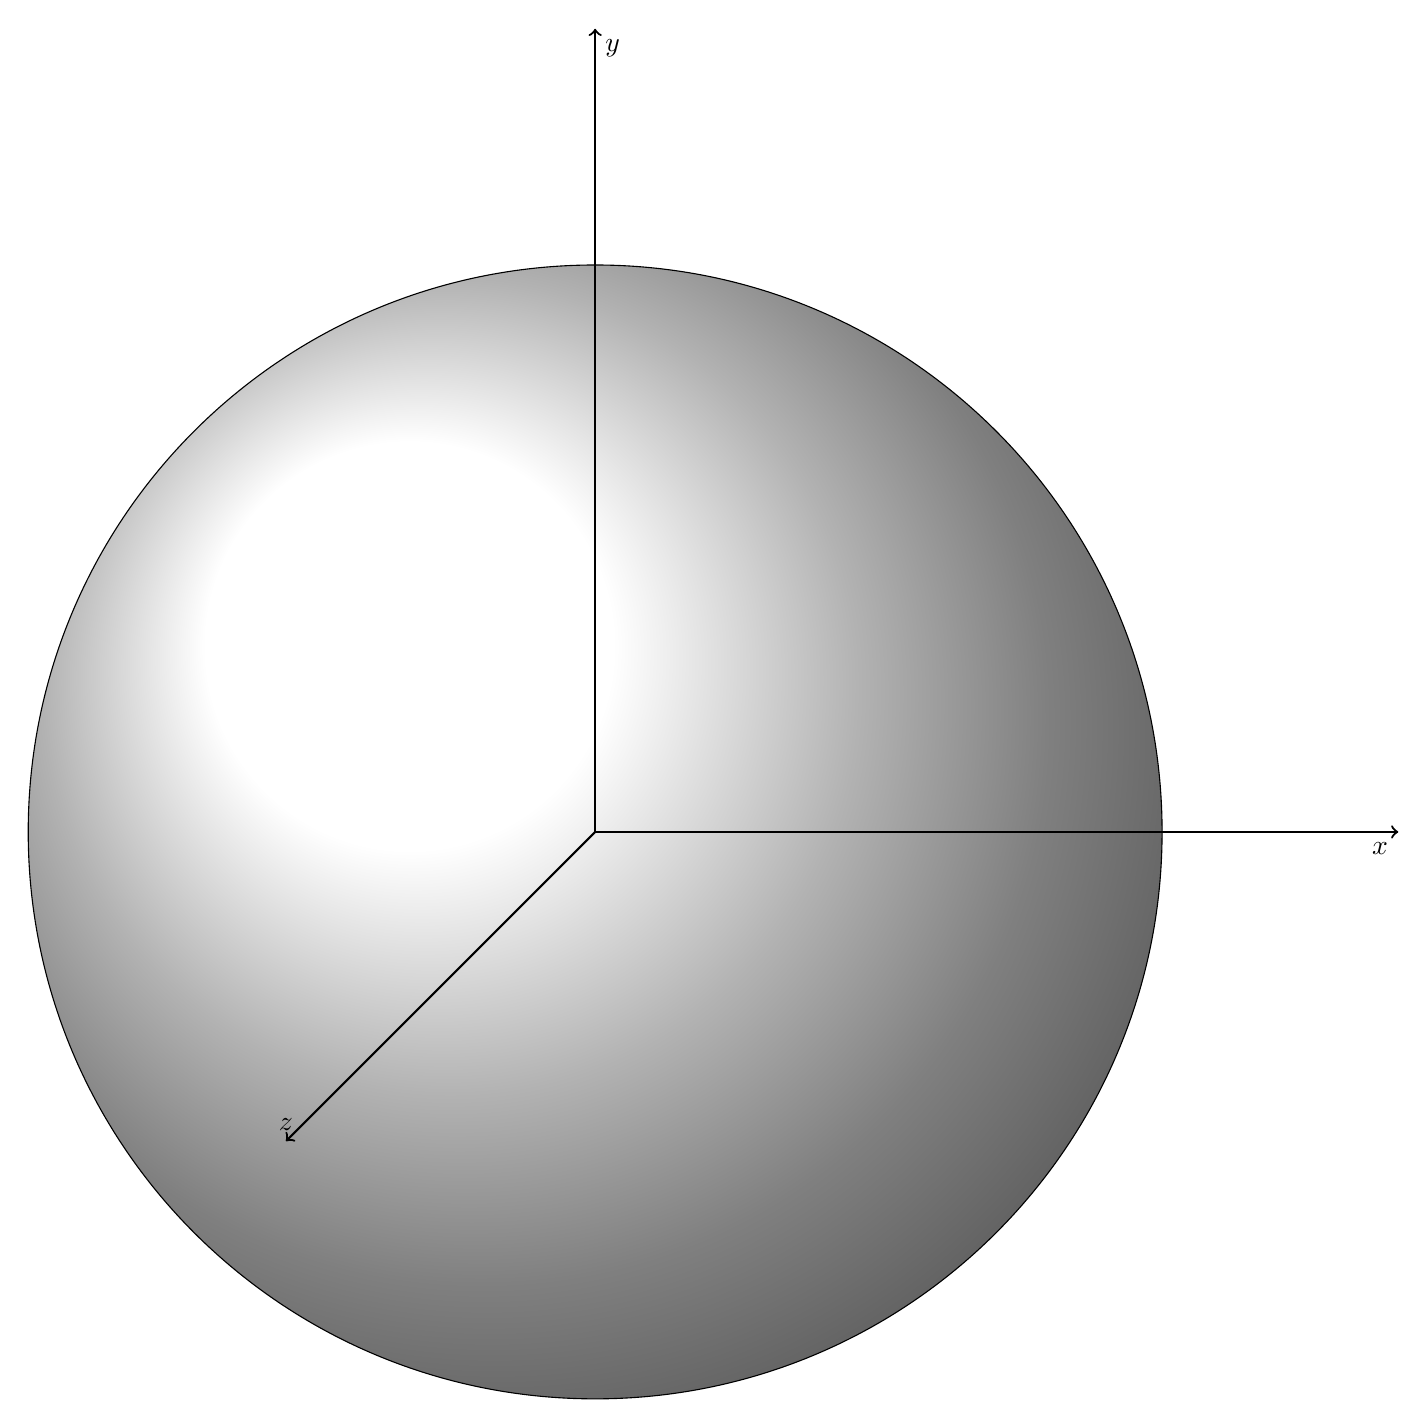
\begin{tikzpicture}[scale=6]

    % DRAW SPHERE
    \shadedraw[tdplot_screen_coords, ball color = white] (0,0) circle (1.2);

    % DRAW X, Y, Z AXIS
    \draw[thick,->] (0,0,0) -- (1.7,0,0) node[anchor=north east]{$x$};
    \draw[thick,->] (0,0,0) -- (0,1.7,0) node[anchor=north west]{$y$};
    \draw[thick,->] (0,0,0) -- (0,0,1.7) node[anchor=south]{$z$};

\end{tikzpicture}

\end{document}
